\chapter{Эксперименты}

\section{Кросс валидация}
Так как в нашем распоряжении было не много размеченных данных, для исключения
переобучения использовалась кросс валидация. Как было описано ранее, предметным
специалистом были предоставлены примерно одинаковые по продолжительности записи
с разных экспериментов, в связи с чем было логично сделать разбиение на группы
именно по ним. Таким образом, всего у нас получилось 8 групп --- по 1 на
валидацию и тестирование и по 6 на обучение. Всего производилось 8
экспериментов (по одному на уникальную тестовую группу). Валидационная группа
выбиралась случайным образом. Метрики замерялись после обучения на тестовой
группе. В качестве финальной метрики бралось среднее от всех экспериментов.

\section{Результаты}

В определенный момент времени возникла потребность в ручной проверке и
корректировке истинной разметки. Таким образом, у нас появилась более
качественная разметка, на основе которой были измерены метрики. В таблице
\ref{tab:results} показано сравнение результатов работы двух программ: той,
которая описана в данной работе, и той, с помощью которой был выполнен
первоначальный анализ. Для более наглядного сопоставления приведен график
итоговой метрики $F_1score$ на рис. \ref{fig:f1score-vs}.

Как показывает сравнение, удалось достичь повышения качества работы на 11\%,
причем данный подход отличается от оригинальной программы тем, что полностью
автоматизирован и не требует тонкой настройки специалистом.

\begin{table}[ht]
\centering
\label{tab:results}
	\begin{tabular}{ccccccc} \toprule
		& \multicolumn{2}{c}{Precision} & \multicolumn{2}{c}{Recall} & \multicolumn{2}{c}{F1-score} \\
		\textbf{Эксперимент}& \textbf{O} & \textbf{P}& \textbf{O} & \textbf{P}& \textbf{O} & \textbf{P} \\ \midrule
		22ph0               & 0.98837                & 0.98978               & 0.98445             & 0.98777            & 0.98641                  & 0.98877                  \\
		22ph1               & 0.98296                & 0.71065               & 0.45197             & 0.92843            & 0.61922                  & 0.80507                  \\
		23ph0               & 0.97825                & 0.97593               & 0.88805             & 0.96674            & 0.93097                  & 0.97131                  \\
		23ph1               & 0.96247                & 0.84946               & 0.38016             & 0.63552            & 0.54504                  & 0.72708                  \\
		25ph0               & 0.96412                & 0.75438               & 0.84612             & 0.99047            & 0.90128                  & 0.85645                  \\
		25ph1               & 0.37485                & 0.77875               & 0.85144             & 0.93807            & 0.52054                  & 0.85102                  \\
		26ph0               & 0.99379                & 0.83584               & 0.70904             & 0.96802            & 0.82761                  & 0.89709                  \\
		26ph1               & 0.98798                & 0.58380               & 0.38471             & 0.87136            & 0.55378                  & 0.69917                  \\ \midrule
		\textbf{Среднее}    & 0.91848                & 0.81700               & 0.69786             & 0.90254            & 0.73339                  & 0.84638                  \\ \bottomrule
	\end{tabular}
\caption{\centering Результаты экспериментов. O --- оригинальная разметка, P --- предсказанная}
\end{table}

\begin{figure}[!htb]
	\centering
	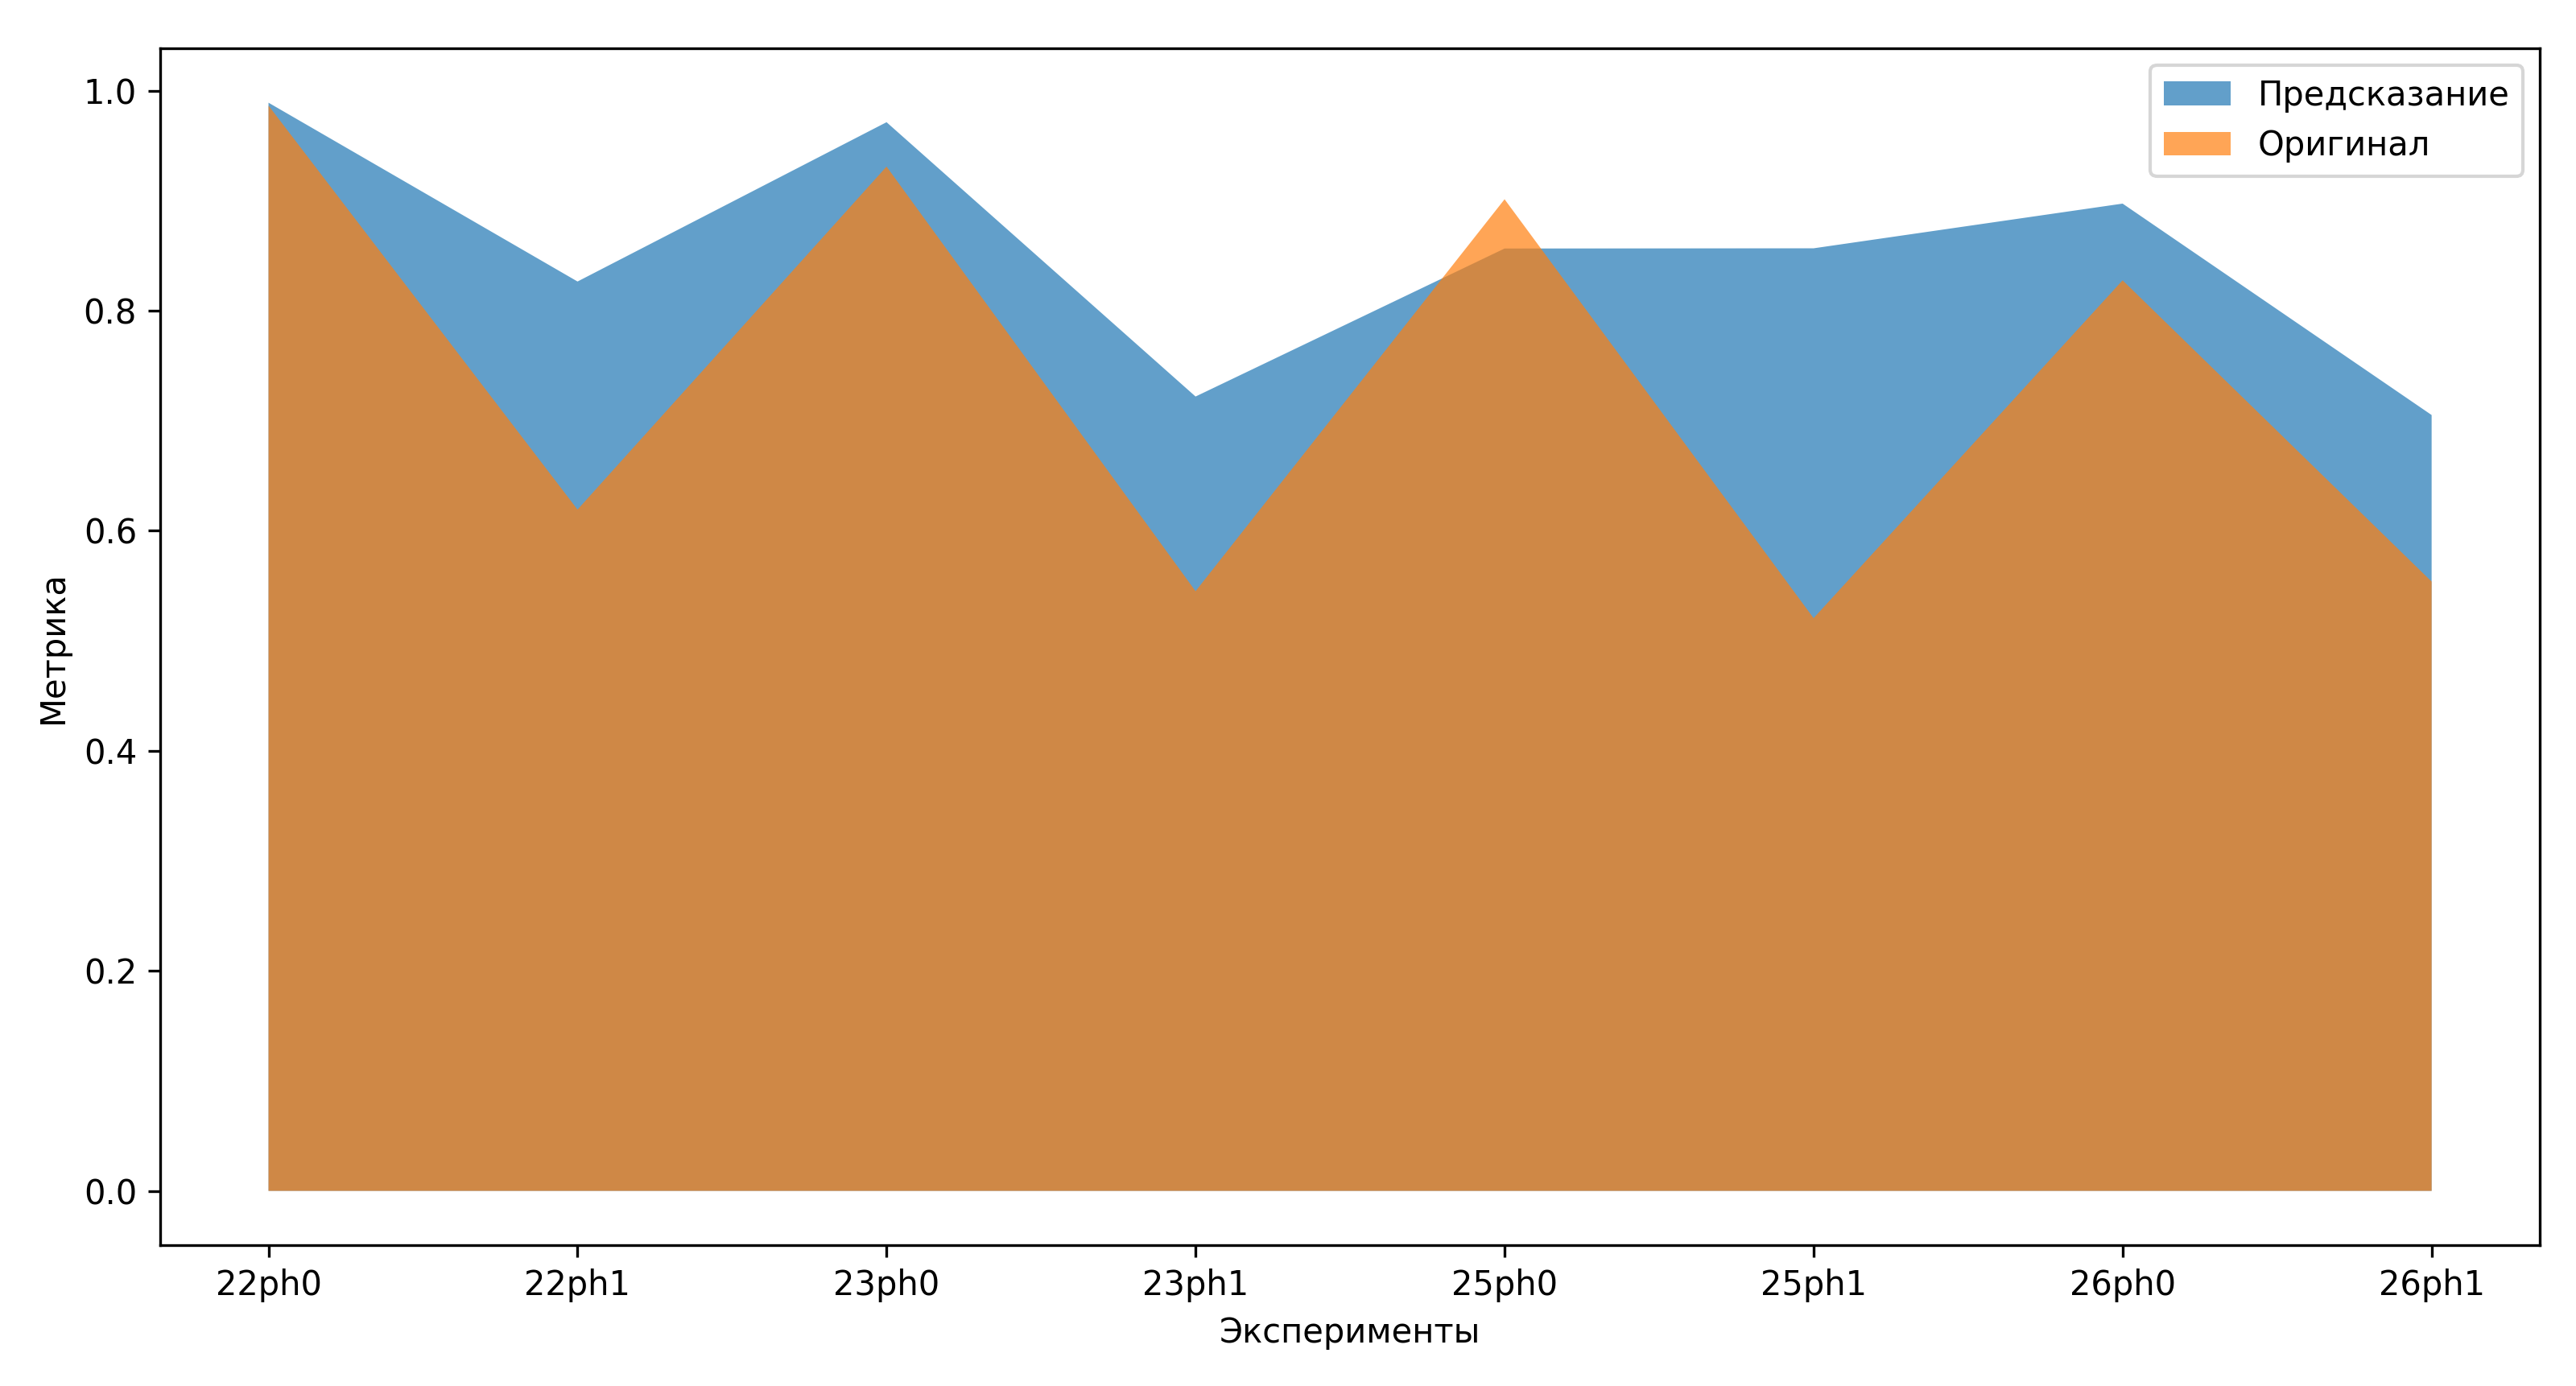
\includegraphics[width=\textwidth]{f1score-cropped.png}
	\caption{Сравнение $F_1score$ оригинальной разметки и предсказанной}
	\label{fig:f1score-vs}
\end{figure}
